% !TEX endcoding = UTF-8 Unicode
% !TEX TS-program = pdflatex
% !TEX spellcheck = en_US

\documentclass[a4paper, 12pt, oneside]{book}
\usepackage[T1]{fontenc}
\usepackage[utf8]{inputenc}
\usepackage[ italian, english]{babel}% la priorità è data all'ultima lingua
\usepackage{verbatim}
\usepackage{geometry}
\geometry{a4paper, top=4cm, bottom=2.5cm, left=3cm, right=3cm, heightrounded, bindingoffset=0mm}
\usepackage{graphicx}
\usepackage{caption}
\captionsetup{tableposition=top, figureposition=bottom, font=small}
\captionsetup{format=hang, labelfont={sf, bf}}
\usepackage{fancyhdr}
\usepackage{booktabs}
\usepackage{mathtools}
\DeclarePairedDelimiter{\abs}{\lvert}{\rvert}
\usepackage{subfig}
\usepackage{amsfonts}
\usepackage{bbold}
\usepackage{braket}
\usepackage{amsmath,bm}
\usepackage{amssymb}
\usepackage{microtype}
\usepackage{bigstrut}
\usepackage{mathrsfs}
\usepackage{multirow}
\usepackage{wasysym}
\usepackage{feynmf}
\usepackage{epstopdf}
\usepackage{rotating}
\usepackage{hyperref}
\usepackage{helvet}
\usepackage{multirow}
\RequirePackage{xspace}
\usepackage{xcolor}
\usepackage{afterpage}
\usepackage{pdfpages}
\usepackage{gensymb}


\begin{document}

\includepdf{frontespizio.pdf} %aggiunge frontespizio
\setcounter{page}{1}
\pagenumbering{roman}
\tableofcontents %%indice

\chapter*{Introduction}
\setcounter{page}{1}
\pagenumbering{arabic}

\addcontentsline{toc}{chapter}{Introduction}
\markboth{}{}
\label{ch:Introduction}
Naples is the city where I was born. It is in Italy and is a wonderful city, near the sea and with a mild climate.\\ 

In this city you can eat very good food everywhere, from pizza to pasta and thousand of different cakes.\\ 

It is a city of art, full of museums and churches where you can find different art styles as Baroque, Neoclassicism and Romantic.\\

It is historic since the city was conquered by different population in the past as Angevin and Aragonese.\\ 

The people are very kind with everyone and it is an alive city also for night life.\\

It is a city of culture, indeed, there are different universities which are very important as University Federico II that is one of the oldest in the world.\\

The site Teleport (\cite{Teleport}) asserts:
\begin{quote}
\textit{Naples, Italy, is characterized by reasonably priced housing. Our data reflects that this city has a good ranking in health-care and tolerance}.
\end{quote}
The site also considers Naples as 17th from a total of 163 countries for what each country on earth contributes to the common good of humanity, and what it takes away, relative to its size.\\

The mayor is trying to give an impulse to the city. He is facing the criminality and dealing with public debt, aiming to increment tourism. In the $2014$ and $2013$ he could get the charge to host respectively the \textbf{Copa Davis} and \textbf{Copa America}.\\

Naples is a city with a very high density of population so it could be a good investment for a local as a restaurant, or hotels, or pizza shop, coffee shop.\\

I want to use data to show what is the best area for an investment by stakeholders in these city.

\chapter*{Data Requirements}
\addcontentsline{toc}{chapter}{Data Requirements}
\label{ch:dataRequirements}
Naples is structured in Municipalities and Neighborhoods. There are 10 municipalities and 31 neighborhoods. I want to find the best area for an investment in commercial area. So I want to get the venues for every municipality, do a clustering of municipalities according their venues and then find the area. Mainly I need for this geospatial data. In particular, the data I will need for my notebook are:\\
\begin{itemize}
\item[-] Data for economy of the city. I will use BeautifulSoap\footnote{BeutifulSoap is a powerful Python library for scraping website} to scrape these data from Wikipedia \cite{economics};

\item[-] Data for municipality and neighborhoods. I will use BeautifulSoap to scrape these data from Wikipedia\cite{municipalities};

\item[-] Data for boundaris of every municipality. I will download the data from open data of the website of the city\cite{opendata}. These data are in the shapefile format. This format is a GIS (Geospatial Information System) standard for geospatial data. Every data is described in the standard WKT (Well Known Text) that describes an element of a map with Point, Linestring, Polygon. In this case the data are polygons that are difficult to manipulate. Yet, from polygons is possible to extract the boundaries as Linestring and the centroids as Point. I did this with an open-source tool QGIS. With shapefiles of boundaries and centroids it is easier to visualize Municipalities on Folium\footnote{Folium is a Python library to visualize geospatial data on a map} map. In figure \ref{fig:qgis_boundaries} you can see an example of what I mean.;

\item[-] Data for climate of the city. Being a city of sun, with a good climate, it is full of tourists the whole year. I will scrape them from a site\cite{climate} with BeautifulSoap;

\item[-] Data from Foursquare API\footnote{he Foursquare Places API provides location based experiences with diverse information about venues, users, photos, and check-ins } to extract venues for every municipality. The referring point for every municipality is the centroid of the municipality extracted as seen before;

\end{itemize}

\begin{figure}[!htb]
		\centering
		\scalebox{0.3}[0.5]{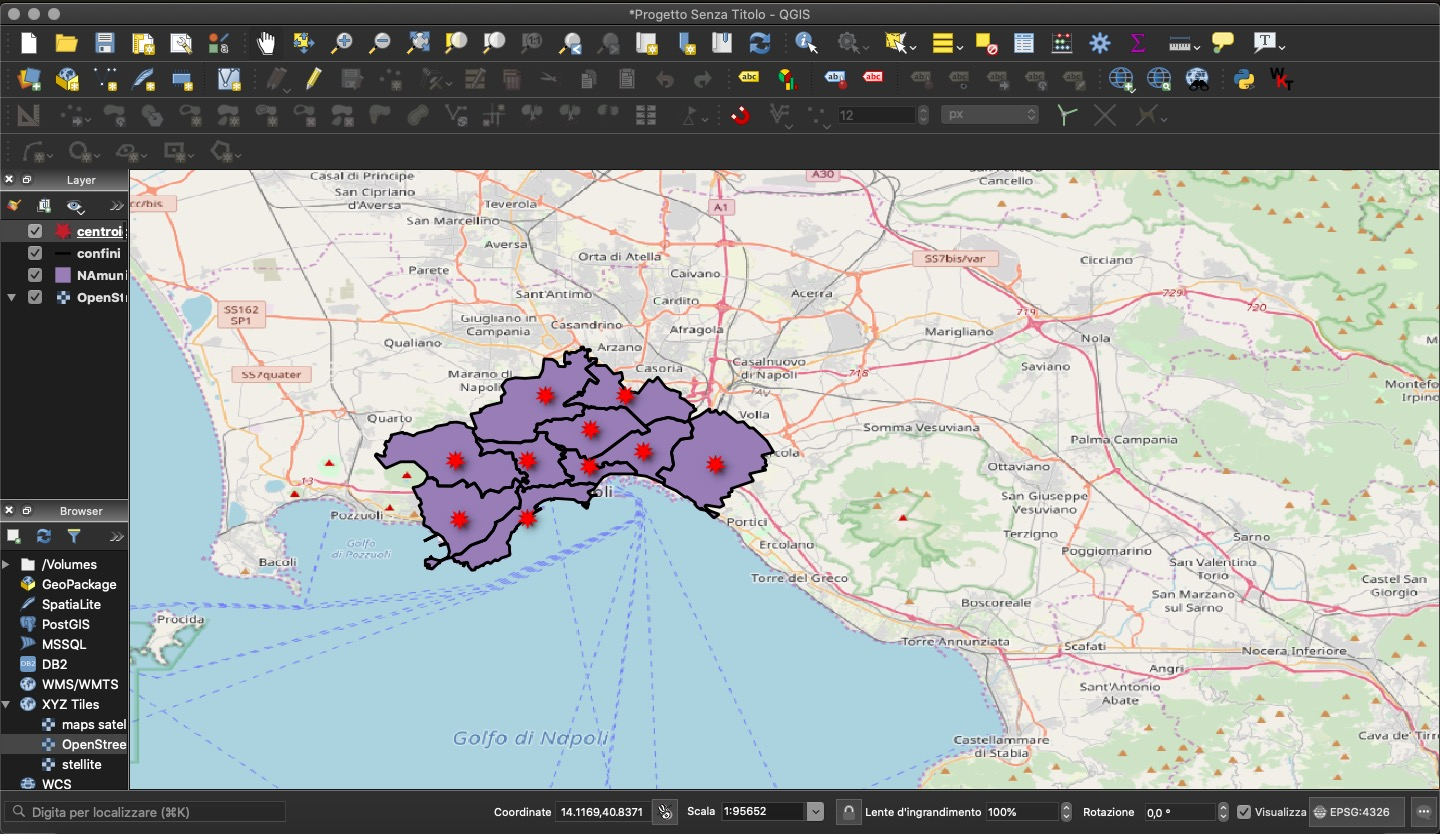
\includegraphics{immagini/qgis_boundaries.jpg}}
		\caption{Example of shapefile imported in QGIS. In violet the polygons representing the municipalities. In black the boundaries. In red star the centroids. }
		\label{fig:qgis_boundaries}
	\end{figure}



 As I mentioned the idea is to cluster municipality by venues, analyze the features of clusters. Then do a heat-map for the area of investment described previously and for every area find what is the best place to invest using density map or contour map.

\chapter*{Data collection and Understanding}
\addcontentsline{toc}{chapter}{Data Collection and Understanding}
\label{ch:dataCollection}
In this chapter we will see the collection of the data and the analysis of them. It's a fundamental step for preparing to modeling the problem.\\
 
The graphs in this chapter and next will be done using matplotlib, a data visualization library in Python.

\section*{Analyze economy of the city} 
\addcontentsline{toc}{section}{Analyze economy of the city}
\label{sec:economy_city}
Naples is Italy's fourth-largest economy after Milan, Rome and Turin, and is the world's 103rd-largest urban economy by purchasing power, with an estimated 2011 GDP of US dollar 83.6 billion, equivalent to $\$$ 28749 per-capita. 

Naples is a major cargo terminal, and the port of Naples is one of the Mediterranean's largest and busiest. The city has experienced significant economic growth since World War II.

Naples is a major national and international tourist destination, being one of Italy and Europe's top tourist cities. Tourists began visiting Naples in the 18th century, during the Grand Tour. In terms of international arrivals, Naples was the 166th-most-visited city in the world in 2008, with 381000 visitors (a 1.6 per cent decrease from the previous year), coming after Lille, but overtaking York, Stuttgart, Belgrade and Dallas \cite{economics}.\\

Figure \ref{fig:df_economy} shows how is distributed the economy of the city. Investment in hotel is just $3.7~\%$, commerce $14~\%$ so it could be a good investment in this area since the city is not filled.

\begin{figure}[!htb]
		\centering
		\scalebox{0.45}[0.5]{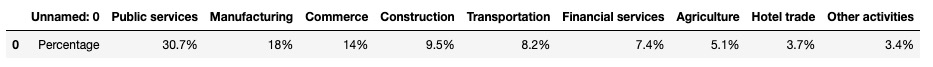
\includegraphics{immagini/dataframe_economics.jpg}}
		\caption{Dataframe describing economy of the city. }
		\label{fig:df_economy}
	\end{figure}
\clearpage

\section*{Build dataframe for Municipalities and Neighborhoods} 
\addcontentsline{toc}{section}{Build dataframe for Municipalities and Neighborhoods}
\label{sec:df_municipality}
The dataset for municipalities and neighborhoods is scraped from Wikipedia\cite{municipalities} using the Python library BeautifulSoap and imported in the notebook as a Pandas dataframe\footnote{Pandas is a fundamental Python library for data analysis. A dataframe is data structure that can be imagined as a table with indices for rows and columns.}. In figure \ref{fig:df_mun_raw} you can see the raw data imported as a dataframe.
This dataset should be cleaned ad adjusted to be usable. Let's drop the columns "Presidente" indicatind the president for municipality (of no use in this case) and "Mappa" which contained the maps of each municipality in Wikipedia as images (clearly the images are not scraped). Then we should add a referring for latitude and longitude of every municipality. For that I download the open-data \cite{opendata} and I extracted the centroids of the polygons of municipalities to get the referring coordinates. As seen in the chapter "Data Requirements" I did it with the open source software QGIS and used the library shapefile of Python to read the centroids saved locally and then updated in my github\cite{dataset}.  

\begin{figure}[!htb]
		\centering
		\scalebox{0.45}[0.5]{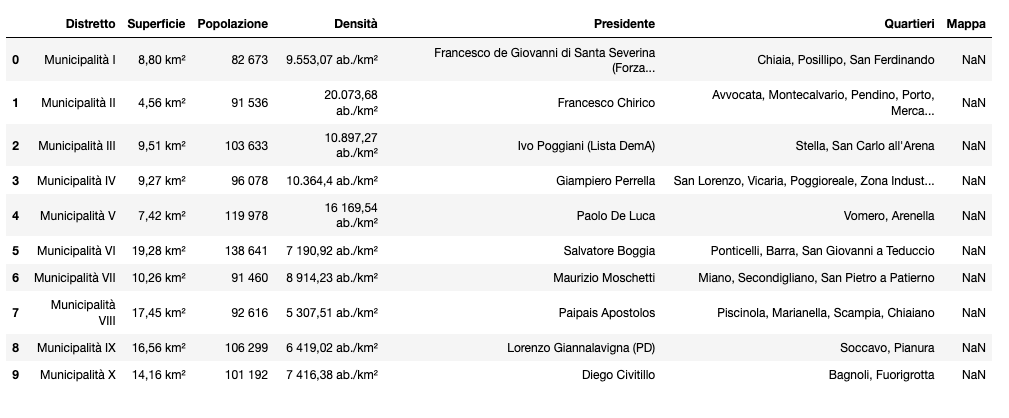
\includegraphics{immagini/df_mun_raw.png}}
		\caption{Dataframe describing raw data for municipalities and neighborhoods. }
		\label{fig:df_mun_raw}
	\end{figure}

After cleaned the dataframe and added latitude, longitude and number neighborhoods for every municipality, it appears as in figure \ref{fig:df_mun_cleaned}


\begin{figure}[!htb]
		\centering
		\scalebox{0.45}[0.5]{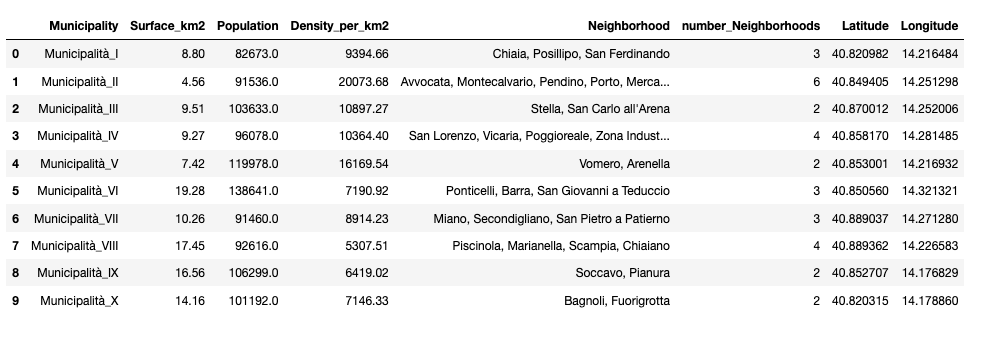
\includegraphics{immagini/df_mun_cleaned.png}}
		\caption{Dataframe describing cleaned data for municipalities and neighborhoods. }
		\label{fig:df_mun_cleaned}
	\end{figure}



Let's import also the boundaries in the same manner as centroids (the dataset is always in my github \cite{dataset}) and plot on the map the data for centroids and boundaries. See figure \ref{fig:map_municipality} showing a Folium map for boundaries and centroids.



\begin{figure}[!htb]
		\centering
		\scalebox{0.45}[0.5]{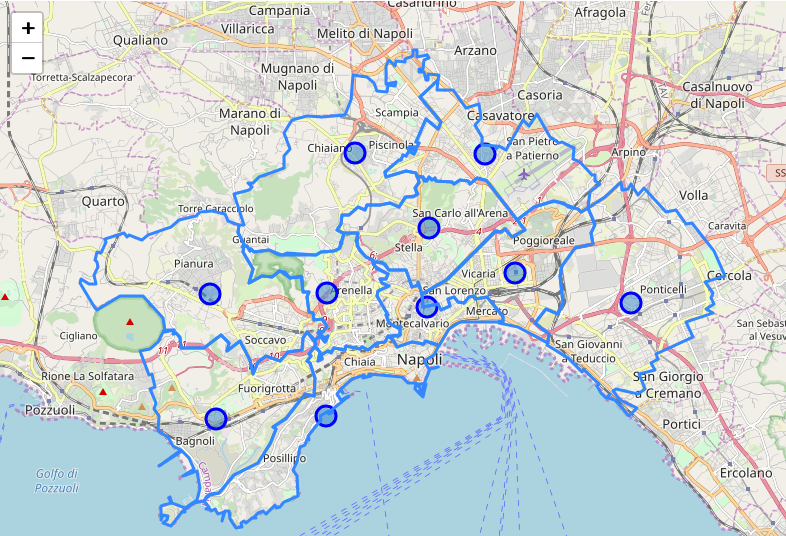
\includegraphics{immagini/map_municipality.png}}
		\caption{A Folium map for municipalities and neighborhoods. }
		\label{fig:map_municipality}
	\end{figure}

\clearpage
\section*{Extract climate data}
 \addcontentsline{toc}{section}{Extract climate data}
\label{sec:climate}
As I mentioned previously, Naples is a city with a very mild climate. Let's see it. I scraped the data from a website \cite{climate} and in figure \ref{fig:df_climate} you can see a dataframe for climate data.



\begin{figure}[!htb]
		\centering
		\scalebox{0.45}[0.5]{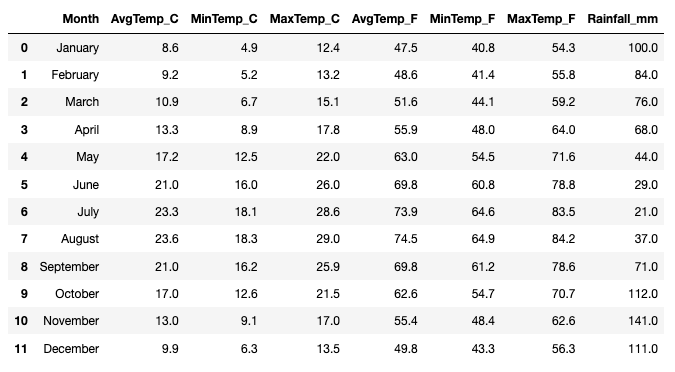
\includegraphics{immagini/df_climate.png}}
		\caption{Climate dataframe for Naples city. }
		\label{fig:df_climate}
	\end{figure}

Let's analyze and visualize these data. 
We can see the trend of temperature in time and by this way also the rainfall in time. 
In figure \ref{fig:np_temp_rain} I reported the trend for averae temperature in degrees centigrade with minimum and maximum variation (left) and a bar plot of the trend for rainfall in mm.

\begin{figure}[!htb]
		\centering
		\scalebox{0.35}[0.4]{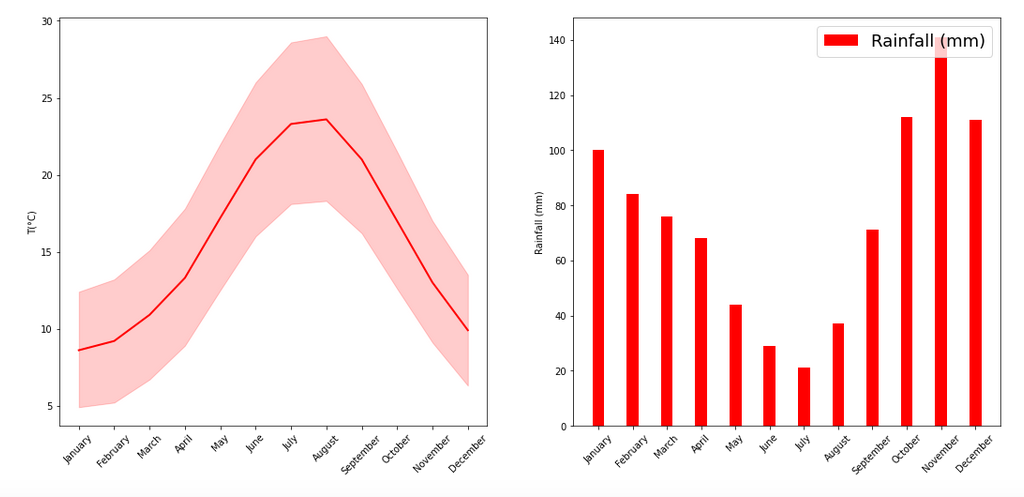
\includegraphics{immagini/np_temp_rain.png}}
		\caption{Trend for average temperature in degrees centigrade (left) and barplot for rainfall in mm (right).}
		\label{fig:np_temp_rain}
	\end{figure}

In order to have a better idea of these data let's do a comparison with another city as New York. In figure \ref{fig:ny_temp_rain} you can see this comparison red for Naples and blu for New York.

\begin{figure}[!htb]
		\centering
		\scalebox{0.35}[0.4]{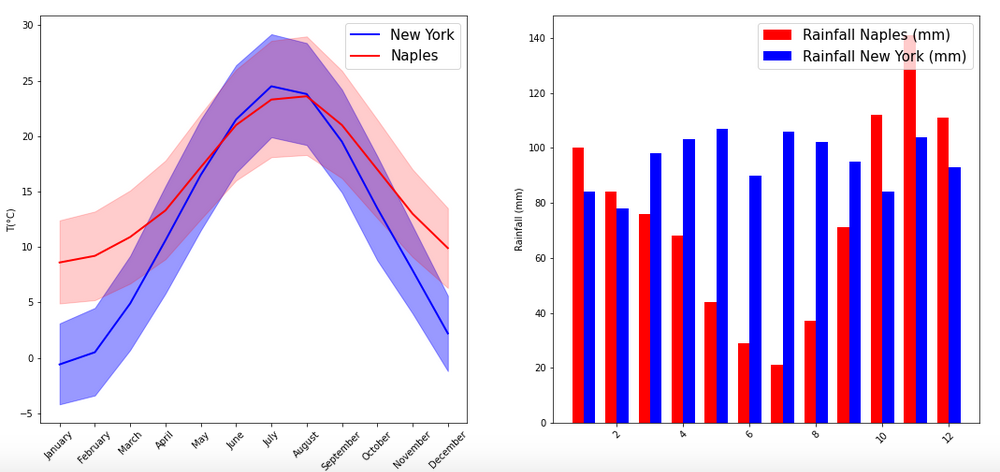
\includegraphics{immagini/ny_temp_rain.png}}
		\caption{Trend for average temperature in degrees centigrade (left) and barplot for rainfall in mm (right).}
		\label{fig:ny_temp_rain}
	\end{figure}

We can see that Naples has generally an higher temperature over $10~ ^{\circ}$C and a lower rainfall than New York.

\section*{Descriptive analysis}
 \addcontentsline{toc}{section}{Descriptive analysis}
\label{sec:descr_analysis}
Let's consider again the dataframe extracted for municipalities and let's do a describe of this dataframe (figure \ref{fig:describe})



\begin{figure}[!htb]
		\centering
		\scalebox{0.45}[0.5]{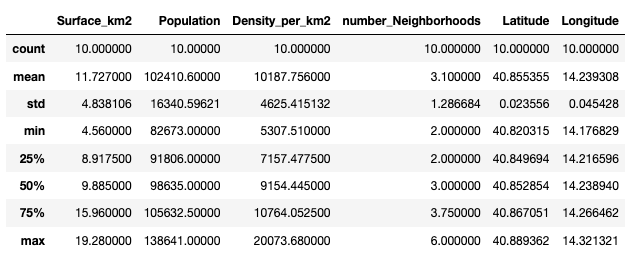
\includegraphics{immagini/describe.png}}
		\caption{A statistical description of the dataframe for municipalities.}
		\label{fig:describe}
	\end{figure}


These data show a mean density of population of $\sim 10000$ people per $km^2$, a very high number for density.

Let's do now some bar plot to deepen these data. 


\begin{figure}[!htb]
		\centering
		\scalebox{0.45}[0.5]{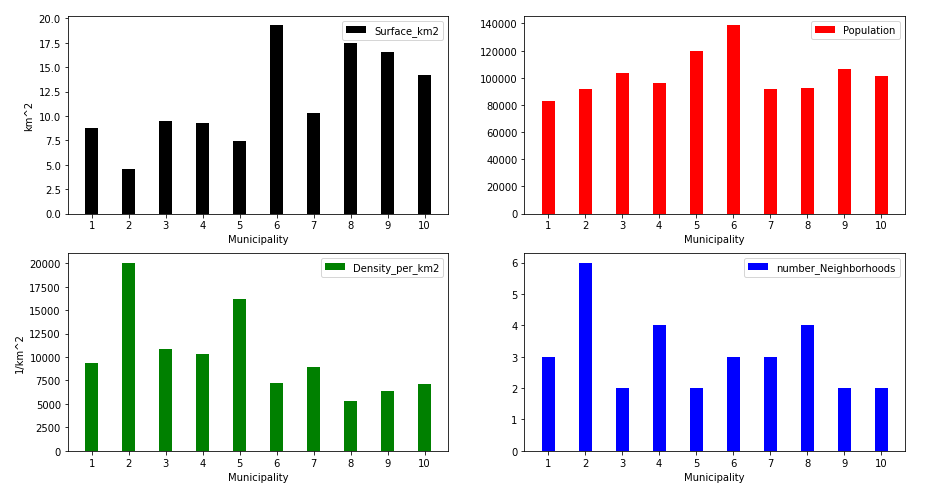
\includegraphics{immagini/barplots.png}}
		\caption{Bar plots for several variables of the dataframe of municipalities.}
		\label{fig:barplots}
	\end{figure}

From the figure \ref{fig:barplots}  we can note that population is concentrated primarily in municipality with lower surface (Black and red graphs up to municipality 5. The black graph grows from municipality 5 while red graph is almost constant). So in this area there is a greater density of population (green graph). There is a greater number of neighborhoods for second municipality that shows 6 neighborhoods and $\sim 20000$ people per $km^2$.
Let's do a scatter plot to better highlight these features. In figure \ref{fig:population_surface} there is a net separation at 12 $km^2$. 

\begin{figure}[!htb]
		\centering
		\scalebox{0.5}[0.55]{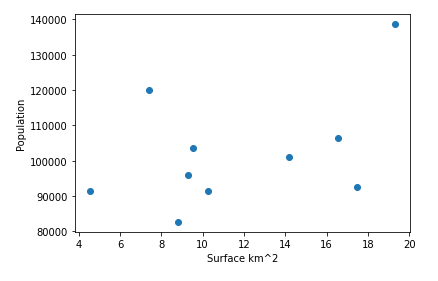
\includegraphics{immagini/population_surface.png}}
		\caption{Scatter plot of Population Versus surface of municipalities.}
		\label{fig:population_surface}
	\end{figure}

If we count the overall population at this cut value we find: 
\begin{itemize}
\item Population in municipality with Surface lower than 12 $km^2$: 585358.
\item Population in municipality with Surface greater than 12 $km^2$: 438748.
\end{itemize}

Since the Municipality II has a surface of $\sim 4~km^2$ and a density in population of $\sim 20\cdot10^3~km^2$ it could be a good candidate for an eventual investment in commerce area. 

\section*{Foursquare API data collection}
 \addcontentsline{toc}{section}{Foursquare API data collection}
\label{sec:foursquare}
Using the Foursquare API I can do some requests to get some information starting from a coordinate. I can do an "explore" query to get all the venues in a certain range starting from a coordinate. Considering every coordinate extracted previously from shapefiles and doing an explore request on the API for each of it we can get all the venues for Naples city according Foursquare. In figure \ref{fig:explore} there is the dataframe with all the venues extracted, the category and coordinates. There are 377 venues. 



\begin{figure}[!htb]
		\centering
		\scalebox{0.45}[0.5]{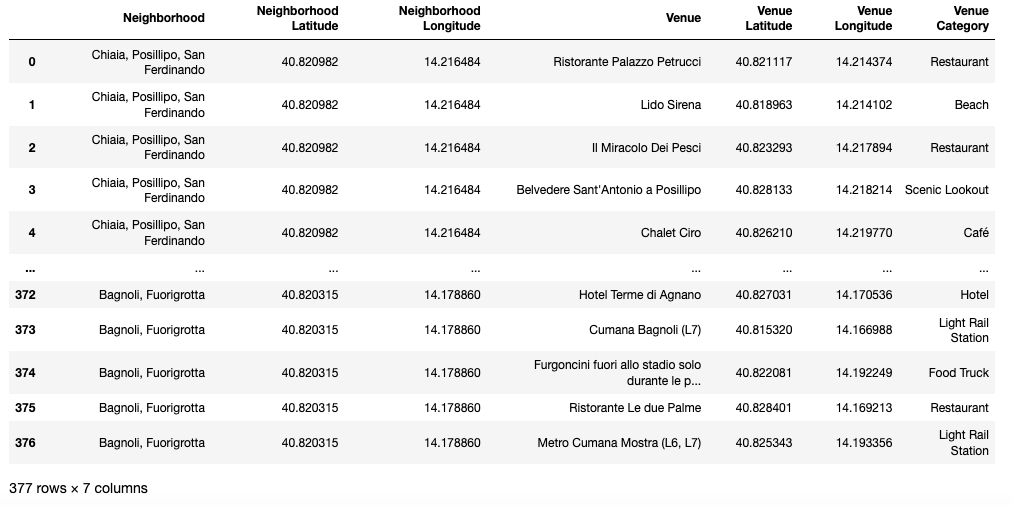
\includegraphics{immagini/explore.png}}
		\caption{Dataframe for venues in Naples city according Foursquare API.}
		\label{fig:explore}
	\end{figure}

Then let's group rows by neighborhood and by taking the mean of the frequency of occurrence of each category. At the end we can display the top 10 venues for each municipality. In figure \ref{fig:venues} is visible a dataframe with venues for all municipalities.\\

\begin{figure}[!htb]
		\centering
		\scalebox{0.5}[0.5]{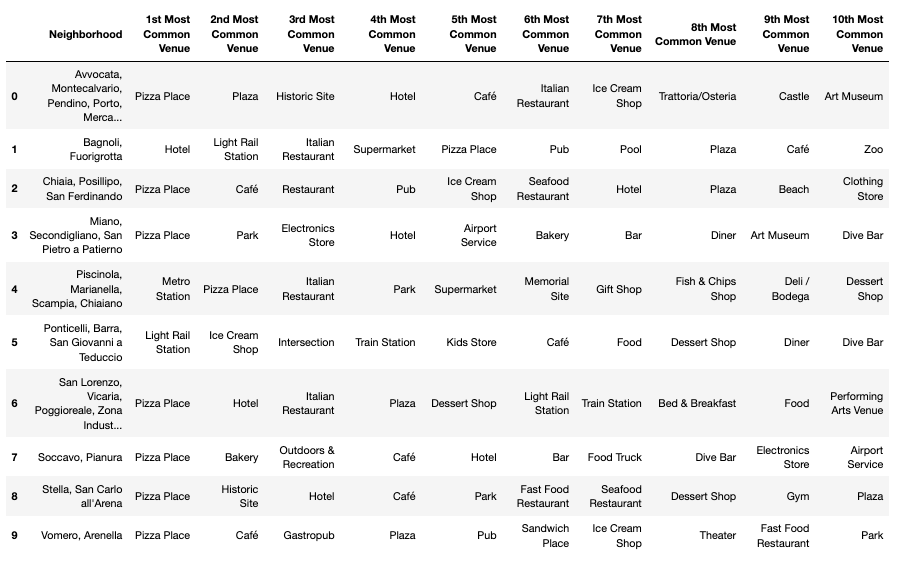
\includegraphics{immagini/venues.png}}
		\caption{Dataframe for top 10 venues for every municipality according Foursquare API.}
		\label{fig:venues}
	\end{figure}


This dataframe concludes the data preparation and now is possible the creation of the model.


\chapter*{Model Clustering Neighborhoods}
\addcontentsline{toc}{chapter}{Model Clustering Neighborhoods}
\label{ch:modelClustering}
The data are modeled using a clustering algorithm. I used a clustering K-means alghoritm. This is a method of vector quantization, originally from signal processing, that aims to partition n observations into k clusters in which each observation belongs to the cluster with the nearest mean (cluster centers or cluster centroid), serving as a prototype of the cluster\cite{clustering}.\\

The centroids are initialized with casual values and updated in an iterative way every time the cluster are determined up to a tolerance value. The problem with this algorithm is it is dependent from the starting points as centroids so it could give different answers every time it is applied.\\

I used the implementation of this algorithm in the Python library Sklearn. 

\section*{Determining the best value for k}
 \addcontentsline{toc}{section}{Determining the best value for k}
\label{sec:k}
In order to find the best k, is applied the Elbow method \cite{elbow} that considers the sum of distances of points from clusters varying the value of the number of clusters k.\\

I did it and the best value for k is 4 as you can see in figure \ref{fig:bestK}



\begin{figure}[!htb]
		\centering
		\scalebox{0.65}[0.65]{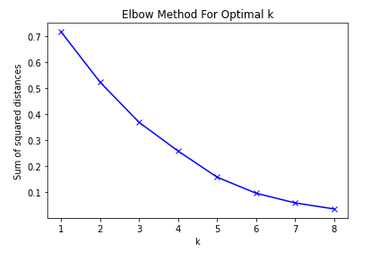
\includegraphics{immagini/bestK.png}}
		\caption{Best value of K for cluster K-means using Elbow method.}
		\label{fig:bestK}
	\end{figure}


\section*{Evaluating the model}
 \addcontentsline{toc}{section}{Evaluating the model}
\label{sec:model_eval}

After having done clustering of the data we can see the clusters on the map and the features they have. Figure, \ref{fig:clusters} shows how municipalities are clusterized.

\begin{figure}[!htb]
		\centering
		\scalebox{0.5}[0.55]{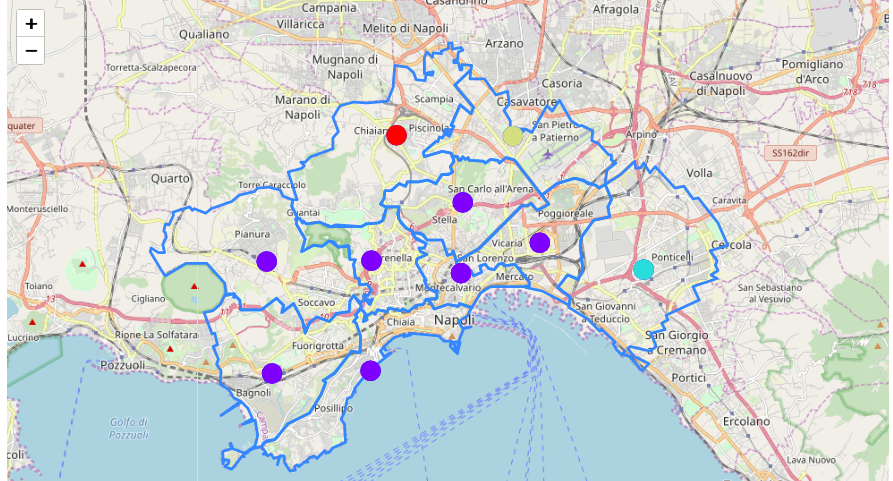
\includegraphics{immagini/clusters.png}}
		\caption{Map showing clusters of municipalities.}
		\label{fig:clusters}
	\end{figure}

The figure shows 3 clusters on the periphery of the city characterized by train stations, parks, supermarkets, bakery.\\

Then there is another big cluster characterized by venues that are hotels, pizza place, coffe and cocktails shop. It is the storic center of the city with museums. It is the part of the city more alive. So it could be a good candidate for an investment. But let's analyze it with more precision in the next chapter. 

\chapter*{Results}
\addcontentsline{toc}{chapter}{Results}
\label{ch:results}

Let's analyze the model in this section. So I employ heatmaps and histo2d to find the "hottest" area for a good investment for an hotel, for a restaurant, for a pizza place or coffee and cocktails shop.\\

For each one of these activities I do a query on Foursquari API for category as "search" to get the venues for every activity.\\

I extract the coordinates of each venue and I do a heatmap with Folium to see where is the hottest zone for a specific category. Then I do 2d histogram, a density plot and a contour plot to get for every activity the best position for the investment.\\

I map the latitude and longitude in a plane (an approximation for little area). Then I get the max for the distributions of latitude and longitude and that could be a reasonable estimation for the most likely position, where the same activities are concentrated.\\

The figure \ref{fig:hotel_density} shows the scatter, histo2d, kde density, contour plots for latitude and longitude, for the category hotel.


\begin{figure}[!htb]
		\centering
		\scalebox{0.5}[0.55]{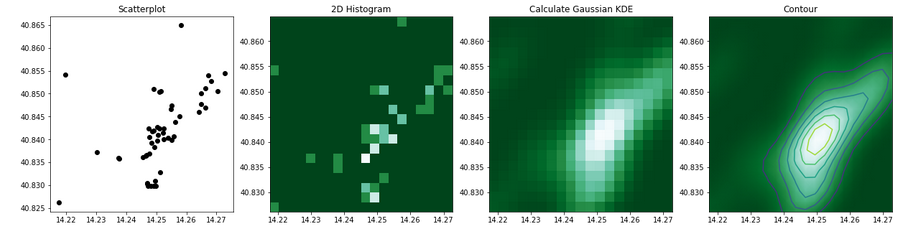
\includegraphics{immagini/hotel_density.png}}
		\caption{Scatter, histo2d, kde density, contour plots for latitude and longitude, for the category hotel.}
		\label{fig:hotel_density}
	\end{figure}
\clearpage
The figure \ref{fig:hotel_map} shows clusters, the heat-map map and the best location (in black) for hotel category.

\begin{figure}[!htb]
		\centering
		\scalebox{0.45}[0.5]{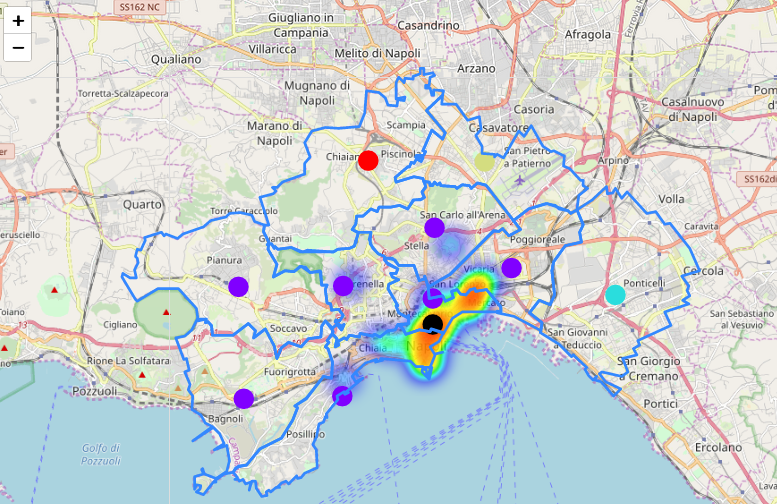
\includegraphics{immagini/hotel_map.png}}
		\caption{Clusters, the heat-map and the best location for hotel category (in black).}
		\label{fig:hotel_map}
	\end{figure}

We can do the same analysis for other categories. I did it for the categories: hotel, pizza, restaurant, coffee, cocktails.\\

In figure \ref{fig:finalResult} I show the best locations.
\begin{figure}[!htb]
		\centering
		\scalebox{0.5}[0.55]{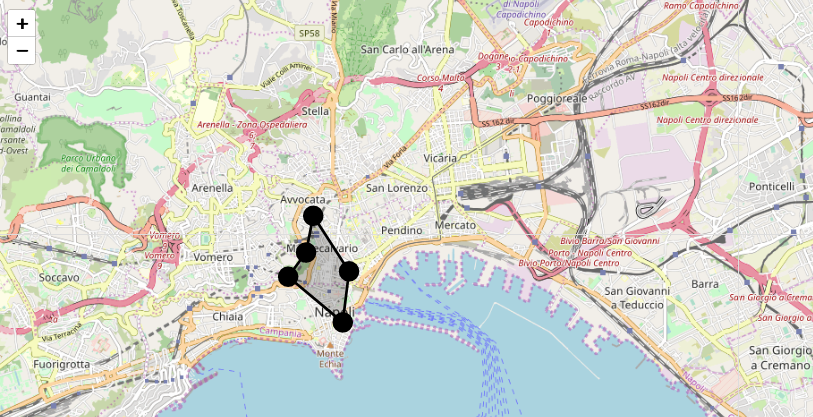
\includegraphics{immagini/finalResult.png}}
		\caption{Best locations for the categories: hotel, pizza, restaurant, coffee, cocktails.}
		\label{fig:finalResult}
	\end{figure}

\clearpage

The points on the map could constitute a polygon for a very reasonable area for a good investment. It is located in municipality 2 which as we considered at the beginning was a good candidate for an investment.
Indeed, it is the historic part of the city, full of museums, it is a short area $\sim 4 ~ km^2$ but with an high density of population 20000 people per $km^2$. It is near the sea and is an attraction for tourists. 


\clearpage
\chapter*{Conclusion}
\addcontentsline{toc}{chapter}{Conclusion}
\label{ch:conclusion}
In this project I analyzed the city where I was born. A beautiful city that needs to be relaunched with tourism, with investments. This is a city with a very good climate, mild. A city of sea, with very good food everywhere you see. It is a city with a very high density of population so everywhere you invest in a local it is always full of people.\\

The city is structured in municipalities and neighborhoods. 
I used open data to get information about municipality, for boundaries and centroids.\\

I used Foursquare API to get data about venues. I clustered municipality. I found 4 clusters. 3 are in the residential zone of the city, made up of train station, parks, bakery, supermarket. 1 of that is full of restaurants, hotels, pizza place, coffee and cocktails shop.\\

I plotted on heat-map these activities and found the best location, that more likely using histo 2d plot and contour plot. \\

I plotted all the best places on a map. These constitute a polygon. That could be a very reasonable area fora good investment. \\

This area is located in Municipality 2, the shortest with 4 squared kilometers but with a very very high density of population, ~20000 people per squared kilometer. \\

The analysis can be further extended going to consider other categories as food, gym or deepen those already considered as doing a research for a better location of Italian restaurant, Chinese restaurant and so on.

\begin{thebibliography}{9}
\bibitem{Teleport} 
https://teleport.org/cities/naples/
 
\bibitem{economics}
https://en.wikipedia.org/wiki/Naples

\bibitem{municipalities}
https://it.wikipedia.org/wiki/Municipalit$\%$C3$\%$A0$\_$di$\_$Napoli

\bibitem{opendata}
http://www.comune.napoli.it/flex/cm/pages/ServeBLOB.php/L/IT/IDPagina/26531 

\bibitem{climate}
https://en.climate-data.org/europe/italy/campania/naples-4561/

\bibitem{dataset}
https://github.com/claudio$-$calamita/Coursera$\_$Capstone/tree/master/dataset

\bibitem{clustering}
https://en.wikipedia.org/wiki/K$-$means$\_$clustering

\bibitem{elbow}
https://blog.cambridgespark.com/how-to-determine-the-optimal-number-of-clusters-for-k-means-clustering-14f27070048f
\end{thebibliography}
\end{document}